\scanpage{36}
% archive foliation: 35

\[
(40)\quad
\left\{
\diagram{\begin{array}{lll}
\deleted{\unsure{\underline\omega_\Delta}}\ C_\Delta\ (\text{``couleurs''})
&\mathrm{Or}(\Delta)&
\deleted{\unsure{\mathrm{Aut}_{\mathrm{oct}}(\Delta)}}\\
\substack{\text{ens. des 2 tétraèdres (échangés par l'}\\
\text{antipodisme) inscrits dans le cube}\\
\text{qui correspond à }\Delta}
&
\substack{\text{ens des}\\\text{deux orientations}\\\text{de l'octaèdre }\Delta\\\simeq}
&
\substack{\underline\omega_\Delta=\underline\omega_{I_\Delta}\\
\text{ens. des deux orientations}\\\text{de }I_\Delta,\text{ ou encore,}\\\text{de }J_\Delta}\\
\begin{array}{cl}\figure{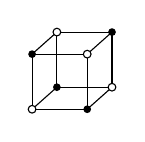
\begin{tikzpicture}[scale=.7]
\draw (0,0)--(1,0)--(1,1)--(0,1)--cycle;
\draw (.45,.4)--(1.45,.4)--(1.45,1.4)--(.45,1.4)--cycle;
\draw (0,0)--(.45,.4) (1,0)--(1.45,.4) (1,1)--(1.45,1.4) (0,1)--(.45,1.4);
\fill (0,1) circle (.07) (1,0) circle (.07) (.45,.4) circle (.07) (1.45,1.4) circle (.07);
\draw[fill=white] (0,0) circle (.07) (1,1) circle (.07) (.45,1.4) circle (.07) (1.45,.4) circle (.07);
\end{tikzpicture}}&\substack{\text{ou encore des}\\
\text{deux couleurs (échangées}\ldots\text{)}\\
\text{des faces de}\\\text{l'octaèdre }\Delta}\end{array}
&
\substack{\text{correspond au car.}\\\text{non trivial de}\\\{1,\underline a_\Delta\}}
&
\substack{\text{correspond}\\\text{au caractère}\\\text{non trivial}\\
\text{de }\mathrm{Aut}_{\mathrm{oct}}^+(\Delta)}\\
\begin{array}{cl}\figure{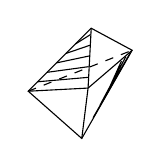
\begin{tikzpicture}[scale=.8]
\draw (0,0)--(1,1)--(1.65,.65)--(.85,-.75)--cycle;
\draw (1,1)--(.95,.05)--(.85,-.75) (0,0)--(.95,.05)--(1.65,.65);
\draw[dashed] (0,0)--(1.65,.65);
\draw (.15,.15)--(.95,.22) (.3,.3)--(.96,.39) (.45,.45)--(.97,.56) (.6,.6)--(.98,.73) (.75,.75)--(.99,.9);
\draw (1.03,-.42)--(1.62,.61) (1.14,-.22)--(1.55,.55) (1.25,-.03)--(1.48,.48);
\end{tikzpicture}}&\substack{\text{correspond.}\\\text{du car. }\deleted{\unsure{\mathrm{sg}\times\det}}\\
\text{de }\mathrm{Aut}_{\mathrm{oct}}^+(\Delta)\times\{1,\underline a_\Delta\}}\end{array}
&&\\
\substack{\uline{\text{NB}}\ \text{On a }F(\Delta)\simeq C_\Delta\times I_\Delta\\
\text{où }I_\Delta=F(\Delta)/\underline a_\Delta\ \text{est l'ens.}\\
\text{des quatre directions de faces}}
&&
\end{array}}
\right.
\]



qui satisfont à un iso. canonique
\[
(41)\qquad
\deleted{\unsure{\mathrm{Or}_\Delta}}\ \mathrm{Or}(\Delta)
\wedge\underbrace{\underline\omega_\Delta}\wedge C_\Delta
\simeq1_{\mathbb{F}_2}.
\]

On a un isom.
\[
(42)\quad
\left\{\begin{array}{l}
C_\Delta=\displaystyle\bigwedge_{i\in J}\Delta_i
\quad\text{quotient de }
\overset{\text{torseur sous }\mathbb{F}_2^J}{\overbrace{\displaystyle\prod_{i\in J}\Delta_i=F(\Delta)}}\\
\qquad\text{pour }\ 
\diagram{\begin{tikzcd}
\mathbb{F}_2^J\arrow[r,"\text{(somme)}"]\arrow[d,equal]&\mathbb{F}_2\\
\underset{M_0}{\underbrace{V_J(\mathbb{F}_2)}}\times\mathbb{F}_2&
\end{tikzcd}}\\
\text{i.e.}\quad C_\Delta=
\underset{\substack{(P_M/(M_0\times\unsure{Z|\mathbb{F}_2})\deleted{\unsure{/M_0}}\text{ dans le cas qui nous occupe})\\
\text{correspond au car. }\mathrm{sg}(g)\cdot\det(g)\text{ dans le cas où}\\
\Delta\text{ est défini par un }M)}}
{\underbrace{F(\Delta)/M_0}}
\end{array}\right.
\]
\margin{donc dans ce cas on a $C_\Delta\simeq\underline\mu\wedge\underline\omega$}

\deleted{(40)}
\[
(43)\qquad
\underline\omega_\Delta=\underline\omega_{I_\Delta}=\underline\omega_J
\quad\text{l'ens à deux éléments associé à }J
\]
(correspond au caractère $\mathrm{sg}(g)$ dans le cas d'un $M$)

\[
(44)\qquad
\deleted{\unsure{\underline\omega}}\ \mathrm{Or}(\Delta)
\simeq
\underset{\underline\omega_J}{\underbrace{\underline\omega_\Delta}}\wedge C_\Delta
\]
\margin{(correspond au caractère $\det(g)$ dans le cas d'un $M$) donc
$\boxed{\mathrm{Or}(\Delta)\simeq\underline\mu^{\det}=(\det M)^*}$.}

L'octaèdre \uline{orienté} \inserted{$\Delta^+$} associé à $M$ est défini par le torseur $P_M/\mathbb{F}_2^{\underline\omega}$ sous $M_0=V_J(\mathbb{F}_2)$, i.e. par
